% Einführungs-Vorlesung für den LaTeX-Kurs (2015-08-07)
% Autor: Simon May
% Datum: 2015-08-05

\usepackage[no-math]{fontspec}
\usepackage{polyglossia}
\setdefaultlanguage{german}

\usepackage{silence}
\WarningFilter{csquotes}{Using preliminary 'polyglossia' interface.}
% biblatex-Warnung harmlos, footnote-patching wird nur für "ibid"-Stile gebraucht
% vgl. https://tex.stackexchange.com/questions/202988/beamer-patching-footnotes-warning
%      https://tex.stackexchange.com/questions/108511/gb4e-biblatex-error-patching-footnotes-failed
\WarningFilter{biblatex}{Patching footnotes failed.}

\usepackage{xcolor}
\usepackage{csquotes}
\usepackage{datetime}
\usepackage{siunitx}
\usepackage{ragged2e}
\usepackage{adjustbox}
\usepackage{wrapfig}
\usepackage{hologo}
\usepackage{tikz}
\usepackage{listingsutf8}
\usepackage{xfrac}
\usepackage{microtype}
% subcaption (noch?) inkompatibel mit beamer!
% => "compatibity=false" für subcaption-Paket notwending
% Hier als Ersatz subfig mit "caption=false" verwendet
% vgl. https://tex.stackexchange.com/questions/125579/subcaption-with-beamer
%      https://tex.stackexchange.com/questions/31906/subcaption-package-compatibility-issue
\usepackage[caption=false]{subfig}
\usepackage[backend=biber, style=authortitle]{biblatex}

\usepackage{hyperref}
\usepackage{cleveref}


% --- Beamer-Einstellungen
\usefonttheme{serif} % only math
\setbeamertemplate{caption}[numbered]
\usetheme[secheader]{Boadilla}
\beamertemplatenavigationsymbolsempty

% --- Paket-Einstellungen
% -- csquotes
\MakeOuterQuote{"}
% -- hyperref
% nur URLs einfärben
\colorlet{linkcolor}{blue!35!black}
\hypersetup{unicode, colorlinks, linkcolor=, urlcolor=linkcolor}
% -- siunitx
\sisetup{
	locale=DE,
	separate-uncertainty,
	quotient-mode=fraction,
	per-mode=fraction,
	fraction-function=\sfrac,
	detect-all
}
\AtBeginDocument{\sisetup{math-rm=\mathrm, text-rm=\rmfamily}}
% -- listings
\let\listingsfont\ttfamily
\colorlet{keywordcolor}{purple!60!black}
\colorlet{emphcolor}{teal!70!black}
\colorlet{commentcolor}{green!40!black}
\colorlet{texcsicolor}{blue}
\colorlet{texcsiicolor}{blue!50!black}
\colorlet{bracescolor}{orange!70!black}
\colorlet{dollarcolor}{red}
\definecolor{stringcolor}{RGB}{47, 0, 255}
\lstdefinestyle{mystandard}{
	% Stelle UTF8-Input mit Latin1 dar
	%inputencoding=utf8/latin1,
	% Zeilennummern links
	%numbers=left,
	% Darstellung der Zeilennummern
	numberstyle=\listingsfont,
	% Rahmen (links)
	%frame=L,
	columns=flexible,
	%xleftmargin=0.5cm,
	% Default Schriftart/Größe
	basicstyle=\small\listingsfont,
	% Darstellung für Keywords
	keywordstyle=\color{keywordcolor},
	% Darstellung für betonte Bezeichner
	emphstyle=\color{emphcolor},
	% Darstellung für Kommentare
	commentstyle=\color{commentcolor},
	% Darstellung für Strings
	stringstyle=\color{stringcolor},
	% Darstellung für TeX-Befehle; Stern: mit backslash
	texcsstyle=*\color{texcsicolor},
	texcsstyle=*[2]\color{texcsiicolor},
	% Tab-Breite
	tabsize=4,
	% Leerzeichen in Strings hervorheben
	showstringspaces=false,
	% Tabs hervorheben
	showtabs=false,
	% Leerzeichen hervorheben
	showspaces=false,
	% Alle Leerzeichen behalten
	keepspaces=true,
	% "Normale" Anführungszeichen: ""
	upquote=true,
	% Lange Zeilen aufbrechen
	breaklines=true,
	% Zeilen an Whitespace aufbrechen
	breakatwhitespace=true,
}

\lstset{
	language=[LaTeX]{TeX},
	style=mystandard,
	escapechar=|,
	deletetexcs={begin, end, documentclass, usepackage},
	moretexcs=[2]{begin, end, documentclass, usepackage},
	moretexcs={
		f, latex, Alpha, eps,
		part, chapter, subsection, subsubsection, paragraph, subparagraph, color, text, mathbb, mathcal, includegraphics, cref, autocite, footcite,
		SI, num, si, SIrange, SIlist, m, per, s, squared, cm, nm, MHz, mega, Hz, cubed, tothe, mA, kV
	},
	literate=
		{\$}{\textcolor{dollarcolor}{\$}}1
		{\{}{\textcolor{bracescolor}{\{}}1
		{\}}{\textcolor{bracescolor}{\}}}1,
}
% --- Befehle
\newcommand{\email}[1]{\href{mailto:#1}{\texttt{#1}}}


\addbibresource{res/literatur.bib}

\title{Einführung in \LaTeX}
\subject{\LaTeX-Kurs}
\author[Simon May]{Simon May\texorpdfstring{\\}{, }\email{simon.may@uni-muenster.de}}
\institute{Fachschaft Physik}
\date{\formatdate{7}{8}{2015}}
\titlegraphic{
\includegraphics[width=5cm]{res/logo.pdf}}
\keywords{Physik, Münster, Praktikum, Protokoll, LaTeX}

\begin{document}

\frame{\titlepage}

\begin{frame}
	\begin{center}
		{\Large
		\textbf{Wichtig:} Wenn es Fragen gibt – fragen!
		
		\medskip
		Wenn es zu schnell geht – Bescheid sagen!}
		
		\bigskip
		Der Inhalt ist wegen der geringen Zeit komprimiert, d.\,h.\ man kann sich zunächst etwas überwältigt fühlen\dots
	\end{center}
\end{frame}

\section{Was ist \LaTeX?}
\subsection{\TeX}

\begin{frame}[<+->]
	\frametitle{Was ist \LaTeX?}
	\visible<+->{1978: {\TeX} (Donald E.\ Knuth)}\visible<+->{\textcolor{gray}{; aktuelle Version: 3.14159265}}
	\begin{itemize}
	\item Programm zum guten und präzisen Textsatz von Büchern (insbesondere mit mathematischem Inhalt)
	\item Heute: Viele Erweiterungen; zu Beginn oft verwirrend!
	\item %\hologo{eTeX},
	\hologo{pdfTeX}, \hologo{XeTeX}, \hologo{LuaTeX}
	\item Derzeit am ausgereiftesten/sinnvollsten: \hologo{pdfTeX}
	\end{itemize}
	\begin{block}{}
		\begin{description}
		\item<.->[\hologo{pdfTeX}:] Gibt PDF-Dateien (direkt) aus
		\item[\hologo{XeTeX}:] UTF-8 (Sonderzeichen!) und Zugriff auf alle Schriftarten des Systems
		\item[\hologo{LuaTeX}:] \hologo{XeTeX}-Features + Programmierbarkeit mit Lua
		\end{description}
	\end{block}
\end{frame}

\subsection{\LaTeX}

\begin{frame}[<+->]
	\visible<+->{1980er: {\LaTeX} (Leslie Lamport); aktuelle Version: \LaTeXe}
	\begin{itemize}
	\item Eine Sammlung von selbstdefinierten Befehlen (\enquote{Makros}) in \TeX; soll Benutzung von {\TeX} vereinfachen
	\item Prinzip: "Logisches Markup" – man sagt z.\,B.: "jetzt kommt eine Überschrift" und {\LaTeX} kümmert sich um gutes Aussehen, Abstände, Seitenumbrüche, Inhaltsverzeichnis etc.
	\item Besondere Stärken von \LaTeX:
		\begin{itemize}
		\item Automatische Nummerierung (Gleichungen, Tabellen, Abbildungen\dots) und Verweise
		\item Literaturverwaltung
		\item Automatisches Literaturverzeichnis, Inhaltsverzeichnis, Tabellen- und Abbildungsverzeichnis
		\item Mathematischer Schriftsatz
		\item Programmierbarkeit
		\end{itemize}
	\end{itemize}
	\visible<+->{{\TeX} und {\LaTeX} sind FOSS (freie Software)!}
\end{frame}

\section{Ein erstes \LaTeX-Dokument}
\section{Struktur eines \LaTeX-Dokuments}

\begin{frame}[fragile]
	\frametitle{Struktur eines \LaTeX-Dokuments}
	\lstset{frame=L, numbers=left, xleftmargin=0.5cm}
	\only<+->{}
	\begin{lstlisting}
	\documentclass{scrartcl} |\visible<+->{\normalfont\color{red}\textleftarrow\ Art des Dokuments}|
	
	|\visible<+->{\normalfont\color{red}Hier befindet sich die sogenannte Präambel. Globale Einstellungen und das Verwenden von Paketen (\LaTeX-Erweiterungen) finden hier statt.}|
	
	\begin{document}
	
	|\visible<+->{\normalfont\color{red}Hierhin wird der Inhalt des Dokuments geschrieben.}|
	...
	
	% Dies ist ein Kommentar. Er beginnt mit dem Prozentzeichen
	% "%" und reicht bis zum Ende der Zeile.
	% Er wird von LaTeX ignoriert und taucht im Dokument
	% nicht auf.
	
	\end{document}
	\end{lstlisting}
\end{frame}

\subsection{Eingabe von \LaTeX-Quelltext}

\begin{frame}[<+->][fragile]
	\frametitle{Ganz normaler Text}
	
	\lstset{frame=L, numbers=left, xleftmargin=0.5cm}
	\begin{itemize}
		\item Für Fließtext gibt man in \LaTeX\ eigentlich nur ganz normal seinen Text ein:
		\begin{columns}<.->
			\column{0.5\textwidth}
			\begin{lstlisting}
			\documentclass{scrartcl}
			\begin{document}
			Dies ist ein Beispieltext. Er
			soll das Schreiben von
			Fließtext verdeutlichen.
			Eigentlich kann man seinen
			Text ganz normal eingeben.
			Seitenumbrüche, Blocksatz und
			das Setzen von Bindestrichen
			(letzteres mit dem richtigen
			Paket) geschehen automatisch.
			\end{document}
			\end{lstlisting}
			\column{0.45\textwidth}
			\justifying\rmfamily
			Dies ist ein Beispieltext. Er
			soll das Schreiben von Fließtext
			verdeutlichen. Eigentlich kann
			man seinen Text ganz normal
			eingeben. Seitenumbrüche,
			Blocksatz und das Setzen von
			Bindestrichen (letzteres mit
			dem richtigen Paket) geschehen
			automatisch.
		\end{columns}
		\item aber es gibt doch einige Besonderheiten\dots
	\end{itemize}
\end{frame}

\begin{frame}[<+->][fragile]
	\frametitle{Besonderheiten bei der Eingabe}
	\begin{itemize}
		\item Mehrere Leerzeichen und einzelne Zeilenumbrüche werden ignoriert:
		
		\begin{minipage}[t]{0.45\textwidth}
			\begin{verbatim}
			Ein kleiner        Test
			123
			\end{verbatim}
		\end{minipage}
		\begin{minipage}{0.45\textwidth}
			\justifying\rmfamily
			Ein kleiner        Test
			123
		\end{minipage}
		\item Für einen Zeilenumbruch: "\lstinline!\\!"; für einen neuen Absatz: Leerzeile
		\item Einige spezielle Zeichen können nicht direkt eingegeben werden: \lstinline!# $ ^ & _ { } ~ \ %!
		\item Eingabe durch Hinzufügen von "\lstinline!\!":\footnote<.->{Die \texttt{\{\}} sind notwendig, weil \texttt{\textbackslash\char`\^} und \texttt{\textbackslash\char`\~} für Akzente genutzt werden; "\texttt{\textbackslash\textbackslash}" ist ein Zeilenumbruch, kein \textbackslash.}
		\begin{lstlisting}
		\# \$ \^{} \& \_ \{ \} \~{} \textbackslash{} \%
		\end{lstlisting}
		\rmfamily
		\# \$ \^{} \& \_ \{ \} \~{} \textbackslash{} \%
		\item \lstinline!{}! erzeugen \LaTeX-Gruppen; Beschränkung der Wirkung von Befehlen:
		
		\begin{minipage}[c]{0.45\textwidth}
			\begin{lstlisting}
			{Dieser Text \bfseries
			ist fett} und dieser nicht
			\end{lstlisting}
		\end{minipage}
		\begin{minipage}[c]{0.45\textwidth}
			\justifying\rmfamily
			{Dieser Text \bfseries ist fett} und dieser nicht
		\end{minipage}
	\end{itemize}
\end{frame}

\subsection{Was sind Befehle?}

\begin{frame}[<+->][fragile]
	\frametitle{\LaTeX-Befehle}

	\begin{columns}<.->[c]
		\column{0.6\textwidth}
		\begin{itemize}
			\item Beginnen mit "\lstinline!\!"
			\item Enthalten nur Buchstaben
			\item Können "alleinstehende" Befehle sein: "\lstinline!\LaTeX!" (= \LaTeX)\dots
		\end{itemize}

		\column<2->{0.3\textwidth}
		\adjustbox{width=\textwidth}{
			\begin{lstlisting}
			\documentclass{scrartcl}
		
			\begin{document}
		
			...
			
			\end{document}
			\end{lstlisting}
		}
	\end{columns}
	
	\lstset{frame=none, numbers=none, xleftmargin=0cm}
	\begin{itemize}
		\item \dots oder Parameter in \emph{geschwungenen Klammern} \lstinline!{ }! annehmen:
		\lstinline!\documentclass{scrartcl}!
		\item Befehle sind wie mathematische Funktionen:\\
		\lstinline!\f{a}{b}{c}! $\mathrel{\widehat{=}} f(a, b, c)$
		\item \emph{Optionale} Parameter in eckigen Klammern \verb|[ ]|:
		\lstinline!\documentclass[a4paper]{scrartcl}!
		\item \emph{Umgebungen} wirken auf den enthaltenen Text:
		\lstinline!\begin{document} Text \end{document}!
	\end{itemize}
\end{frame}

\begin{frame}[<+->][fragile]
	\lstset{frame=none, numbers=none, xleftmargin=0cm}
	\begin{itemize}
		\item Vorsicht: Leerzeichen direkt nach einem Befehl ohne Parameter werden ignoriert:

		\begin{minipage}[c]{0.45\textwidth}
			\begin{lstlisting}
			\LaTeX ist super
			\LaTeX\ ist super
			\LaTeX{} ist super
			{\LaTeX} ist super
			\end{lstlisting}
		\end{minipage}
		\begin{minipage}[c]{0.45\textwidth}
			\justifying\rmfamily
			\LaTeX ist super\\
			\LaTeX\ ist super\\
			\LaTeX{} ist super\\
			{\LaTeX} ist super
		\end{minipage}
		\item Abhilfe schaffen ein manuelles Leerzeichen "\lstinline!\ !", eine leere Gruppe danach oder das Umschließen mit einer Gruppe
		\item \LaTeX\ ist case-sensitiv (\lstinline|\LaTeX| $\ne$ \lstinline|\latex|)
	\end{itemize}
\end{frame}

\subsection{Kompilieren}

\begin{frame}[<+->][fragile]
	\frametitle{Was mache ich jetzt mit meinem \LaTeX-Quelltext?}
	
	\begin{itemize}
		\item Der Quelltext wird von \LaTeX\ verarbeitet, um das Ausgabedokument zu erzeugen
		
		\begin{center}
		\tikzstyle{block}=[rectangle, draw, fill=white, text width=5em, text centered, rounded corners]
		\begin{tikzpicture}[node distance=3cm]
		\coordinate (start);
		\node [block] (quelltext) {Quelltext (\texttt{.tex})};
		\node [block, right of=quelltext] (pdflatex) {\texttt{pdflatex}};
		\node [block, right of=pdflatex] (pdf) {PDF-Dokument};
		\draw [->] (quelltext) -- (pdflatex);
		\draw [->] (pdflatex) -- (pdf);
		\end{tikzpicture}
		\end{center}
		\item Das muss u.\,U.\ mehrmals gemacht werden (z.\,B.\ bei Verweisen)
		
		Grund: \LaTeX\ erzeugt beim Kompilieren Hilfsdateien mit Zusatz-Informationen (\texttt{.aux}, \texttt{.out}, \texttt{.toc}\dots)
		\item Kommandozeile: "\verb|pdflatex dokument.tex|"\dots
		\item \dots aber wenn ihr einen guten Editor habt (z.\,B.\ TeXStudio), müsst ihr euch um all das nicht kümmern
	\end{itemize}
\end{frame}

\begin{frame}[<+->][fragile]
	\frametitle{Was tun, wenn das Dokument nicht kompiliert?}
	
	\begin{itemize}
		\item Die Fehlermeldung lesen!
		\item Leider ist die nicht immer hilfreich\dots
		\item Nach Fehlermeldung suchen; oft hilfreich: \url{https://tex.stackexchange.com}
		\item Manchmal steckt der Fehler in (alten) Hilfsdateien! Ohne Bedenken löschbar (einzig wichtige Datei: \texttt{.tex})
		\item Letzter Ausweg: Zeile für Zeile auskommentieren (\lstinline!%!), bis es fehlerfrei kompiliert \textrightarrow\ problematische Stellen finden
		\item Manchmal erkennt man auch an der (halb-)fertigen PDF, wo der Fehler ist
	\end{itemize}
\end{frame}

\section{Grundlegende \LaTeX-Befehle}

\begin{frame}[<+->][fragile]
	\frametitle{Grundlegende \LaTeX-Befehle}
	
	\begin{itemize}
		\item \lstinline!\\!: Zeilenumbruch; \lstinline!\newpage!: Neue Seite
		\item Schriftart
		\begin{itemize}
			\item \lstinline!\textbf{fett}! — {\rmfamily\textbf{fett}}
			\item \lstinline!\textit{kursiv}! — {\rmfamily\textit{kursiv}}
			\item \lstinline!\texttt{Schreibmaschine}! — {\rmfamily\texttt{Schreibmaschine}}
			\item \lstinline!\underline{unterstrichen}! — {\rmfamily\underline{unterstrichen}}
			\item \lstinline!\textsc{Kapitälchen}! — {\rmfamily\textsc{Kapitälchen}}
		\end{itemize}
		\item \lstinline!\begin{center}zentriert\end{center} \begin{flushleft}linksbündig\end{flushleft} \begin{flushright}rechtsbündig\end{flushright}!
		
		{\justifying\rmfamily
		\begin{center}zentriert\end{center}
		\begin{flushleft}linksbündig\end{flushleft}
		\begin{flushright}rechtsbündig\end{flushright}}
	\end{itemize}
\end{frame}

\begin{frame}[<+->][fragile]
	\begin{itemize}
		\item Textgröße: \lstinline!\tiny \scriptsize \footnotesize \small \normalsize \large \Large \LARGE \huge \Huge!
		
		(Achtung: Textgröße gilt, bis sie wieder geändert wird \textrightarrow\ Gruppierung \lstinline!{...}! verwenden!)
		
		{\rmfamily
		\tiny tiny \scriptsize scriptsize \footnotesize footnotesize \small small \normalsize normalsize \large large \Large Large \LARGE LARGE \huge huge \Huge Huge}
		\item Achtung: Nicht zu wild mit Schriftarten (und besonders -Größen) hantieren! Wirkt sonst inkonsistent oder unprofessionell!
		\item Verwendung von Schriftarten etc.\ meist nur zu Beginn des Dokuments, wenn man das Aussehen \emph{global} anpasst. Ansonsten: Aussehen \LaTeX\ überlassen!
	\end{itemize}
\end{frame}

\begin{frame}[<+->][fragile]
	\lstset{frame=none, numbers=none, xleftmargin=0cm}
	\frametitle{Aufzählungen}

	\begin{itemize}
		\item Ungeordnet:

		\adjustbox{scale=0.8}{
		\begin{minipage}[c]{0.45\textwidth}
			\begin{lstlisting}
			\begin{itemize}
		    	\item Ein Punkt
		    	\item Noch ein Punkt
			\end{itemize}
			\end{lstlisting}
		\end{minipage}
		\begin{minipage}[c]{0.45\textwidth}
			\justifying\rmfamily
			\begin{itemize}[<.->]
				\item Ein Punkt
				\item Noch ein Punkt
			\end{itemize}
		\end{minipage}}
		\item Geordnet:
		
		\adjustbox{scale=0.8}{
		\begin{minipage}[c]{0.45\textwidth}
			\begin{lstlisting}
			\begin{enumerate}
			    \item Erster Punkt
			    \item Zweiter Punkt
			\end{enumerate}
			\end{lstlisting}
		\end{minipage}
		\begin{minipage}[c]{0.45\textwidth}
			\justifying\rmfamily
			\begin{enumerate}[<.->]
			    \item Erster Punkt
			    \item Zweiter Punkt
			\end{enumerate}
		\end{minipage}}
		\item Beschreibung:

		\adjustbox{scale=0.8}{
		\begin{minipage}[c]{0.45\textwidth}
			\begin{lstlisting}
			\begin{description}
			    \item[\LaTeX] Ein Textverarbeitungssystem
			    \item[TeXStudio] Editor für \LaTeX-Quelltext
			\end{description}
			\end{lstlisting}
		\end{minipage}
		\begin{minipage}[c]{0.65\textwidth}
			\justifying\rmfamily
			\begin{description}[<.->]
			    \item[\normalcolor\bfseries\LaTeX] Ein Textverarbeitungssystem
			    \item[\normalcolor\bfseries TeXStudio] Editor für \LaTeX-Quelltext
			\end{description}
		\end{minipage}}
	\end{itemize}
\end{frame}

\begin{frame}[<+->][fragile]
	\begin{itemize}
		\item Gliederung
		\begin{itemize}
			\item \lstinline!\part{Teil}!
			\item \lstinline!\chapter{Kapitel}! (nicht bei \texttt{scrartcl})
			\item \lstinline!\section{Abschnitt}!
			\item \lstinline!\subsection{Unterabschnitt}!
			\item \lstinline!\subsubsection{Unterunterabschnitt}!
			\item \lstinline!\paragraph{Absatz}!
			\item \lstinline!\subparagraph{Unterabsatz}!
		\end{itemize}
		\item Überschriften werden automatisch nummeriert und dem Inhaltsverzeichnis hinzugefügt. Möchte man beides nicht, kann man \lstinline!*! anhängen (z.B.\ \lstinline!\section*{Text}!)
		\item \lstinline!\input{datei.tex}!: Die Datei wird exakt an der Stelle in das Dokument eingefügt \textrightarrow\ Übersichtlichkeit im Quelltext!
	\end{itemize}
\end{frame}

\section{Mathematik in \LaTeX}

\begin{frame}[<+->][fragile]
	\frametitle{Mathematik in \LaTeX}
	
	\begin{itemize}
		\item \LaTeX\ unterscheidet zwischen Text- und Mathemodus
		\item Mathematische Befehle nur im Mathemodus möglich!
		\item Umgebungen für den Mathemodus:\footnote<.->{Es gibt noch weitere.}
		\begin{itemize}
			\item \lstinline!$ ... $!: Formel in der Textzeile ("inline")
			
			\lstinline!$a = b + c$!: $a = b + c$
			\item \lstinline!\begin{equation} ... \end{equation}!: Nummerierte, abgesetzte Gleichung
			\item \lstinline!\begin{align} ... \end{align}!: Mehrere nummerierte, abgesetzte, ausgerichtete Gleichungen
		\end{itemize}
		\item Im Mathemodus werden Leerzeichen ignoriert! Jeder Buchstabe wird als Formelzeichen verstanden
		
		\lstinline!$Text in Mathe-Umgebung$!: {\rmfamily$Text in Mathe-Umgebung$}
		\item Ausweg: \lstinline!\text{...}!
		
		\lstinline!$p V = \text{const.}$!: $p V = \text{\rmfamily const.}$
	\end{itemize}
\end{frame}

\begin{frame}[<+->][fragile]
	\frametitle{Mathe-Befehle}
	
	\begin{itemize}
		\item Nummerierte Gleichung: \lstinline!\begin{equation} E = m c^2 \end{equation}!

		Ergebnis:
		\begin{equation}
		E = m c^2
		\end{equation}
		\item \lstinline!a^n! ergibt $a^n$
		\item \lstinline!n_i! ergibt $n_i$
		\item Was ist mit \lstinline!U_ind!? \textrightarrow\ $U_ind$
		\begin{itemize}
			\item Klammern setzen!\footnote<.->{\lstinline!^! und \lstinline!_! sind eigentlich Befehle; ohne Klammern wird das nächste Zeichen als Parameter verwendet.} \lstinline!U_{ind}! \textrightarrow~$U_{ind}$
			\item Noch besser: \lstinline!U_\text{ind}! \textrightarrow~$U_\text{\rmfamily ind}$
		\end{itemize}
		\item \lstinline!\frac{a}{b}! ergibt $\displaystyle\frac{a}{b}$
		\item \lstinline!\cdot! ist der Malpunkt $\cdot$ (\emph{nicht} \lstinline!*! verwenden!), \lstinline!\times! das Kreuz $\times$
		\item \lstinline!\sqrt{abc}! ergibt $\sqrt{abc}$
	\end{itemize}
\end{frame}

\begin{frame}[<+->][fragile]
	\begin{itemize}
		\item \lstinline!\vec{r}! ergibt $\vec{r}$
		\item \lstinline!\dot{r}! ergibt $\dot{r}$, \lstinline!\ddot{r}! ergibt $\ddot{r}$
		\item Griechische Buchstaben: "\lstinline!\!" + Name des Buchstabens
		\begin{itemize}
			\item Anfangsbuchstabe klein: kleiner Buchstabe; \lstinline!\gamma! \textrightarrow\ $\gamma$
			\item Anfangsbuchstabe groß: großer Buchstabe; \lstinline!\Gamma! \textrightarrow\ $\Gamma$
		\end{itemize}
		\item Warum gibt es kein \lstinline!\Alpha!?
		\item \lstinline!\sum_{n = 0}^{\infty}! \textrightarrow\ $\displaystyle\sum_{n=0}^{\infty}$, \lstinline!\int_{-\infty}^{\infty}! \textrightarrow\ $\displaystyle\int_{-\infty}^{\infty}$
		\item Komplizierteres Beispiel:\footnote<.->{\texttt{\textbackslash begin\{equation*\}}: Wie \texttt{\textbackslash begin\{equation\}}, aber ohne Nummer (vgl.\ \texttt{\textbackslash section*\{\}}).}
		\begin{lstlisting}
		\begin{equation*}
		    \vec{F} = -G \cdot \frac{m_1 m_2 \vec{r}}{r^3}
		\end{equation*}
		\end{lstlisting}
		\begin{equation*}
			\vec{F} = -G \cdot \frac{m_1 m_2 \vec{r}}{r^3}
		\end{equation*}
	\end{itemize}
\end{frame}

\begin{frame}[<+->][fragile]
	\begin{itemize}
		\item Klammern: \lstinline!(\frac{U}{I})! \textrightarrow~$\displaystyle(\frac{U}{I})$ \textrightarrow~Schlecht!
		\item Mit \lstinline!\left(! und \lstinline!\right)!: automatische Größe
		
		\lstinline!\left(\frac{U}{I}\right)! \textrightarrow\ $\displaystyle\left(\frac{U}{I}\right)$
		\item Geht auch mit \lstinline![ ]!, \lstinline!\{ \}!, \lstinline!< >!
		\item \emph{Wichtig:} Es muss ein \lstinline!\left! \emph{und} ein \lstinline!\right! geben! (Müssen aber nicht die gleichen Zeichen sein)
		\item Es gibt spezielle Mathe-Schriftarten
		\item \lstinline!\mathbb{BUCHSTABE}! (nur Großbuchstaben)
		
		$\mathbb{ABCDEFGHIJKLMNOPQRSTUVWXYZ}$ (z.\,B.\ $\mathbb{R}^n$)
		\item \lstinline!\mathcal{BUCHSTABE}! (nur Großbuchstaben)
		
		$\mathcal{ABCDEFGHIJKLMNOPQRSTUVWXYZ}$\\
		(z.\,B.\ Fouriertransformation $\mathcal{F}\{f(t)\}$)
		
		\item Weitere Symbole findet man in der Seitenleiste von TeXStudio!
		\item Man kann sich zu Beginn nicht alles merken! Greift auf die Hilfen eures Editors (TeXStudio) zurück!
	\end{itemize}
\end{frame}

\begin{frame}[<+->][fragile]
	\frametitle{Mathematische Feinheiten}
	\begin{itemize}
		\item Wörter in Mathe-Umgebung mit \lstinline!\text{...}! eingeben (s.\,o.)
		\item Bei Indizes, die sich auf Namen/Wörter und nicht auf Formelzeichen beziehen, bitte \lstinline!\text{...}! verwenden (s.\,o.)!
		\begin{itemize}
			\item Fermi-Energie $E_\text{\rmfamily F}$ statt $E_F$
			\item Aber: Epsilon-Tensor $\varepsilon_{ijk}$
		\end{itemize}
		\item Für "längere" Funktionsnamen gibt es Befehle:
		
		\lstinline!\sin x! \textrightarrow~$\sin x$
		
		\lstinline!sin x! \textrightarrow~$sin x = s \cdot i \cdot n \cdot x$ (falsch!)
		\item Es gibt keine x-Achse, nur eine $x$-Achse!
		\item Das $\mathrm{d}$ bei Differentialen ($\mathrm{d}x$) aufrecht!\footnote<.->{\texttt{\textbackslash,} ist ein kleiner Abstand.}
		
		\lstinline!\int f(x) \, \mathrm{d}x! \textrightarrow\ $\displaystyle\int f(x) \, \mathrm{d}x$
		
		\lstinline!\frac{\mathrm{d}f}{\mathrm{d}x}! \textrightarrow~$\displaystyle\frac{\mathrm{d}f}{\mathrm{d}x}$
		\item Einheiten aufrecht: {\rmfamily$\SI{2}{\kg} > \SI{1}{\kg}$} (für Einheiten gibt es ein \LaTeX-Paket)
	\end{itemize}
\end{frame}

\begin{frame}[<+->][fragile]
	\frametitle{Zusammengehörige Gleichungen}
	\lstset{numbers=left, frame=L}
	\begin{itemize}
		\item Zusammengehörige Gleichungen: \lstinline!\begin{align} ... \end{align}!
		\item "\lstinline!\\!": Neue Gleichung, "\lstinline!&!": Ausrichtung der Gleichungen
		
		\adjustbox{scale=0.8}{
		\begin{visibleenv}<+->
		\begin{minipage}[c]{0.65\textwidth}
			\begin{lstlisting}
			\begin{align}
			\nabla \cdot \vec{E} &= \frac{\rho}{\varepsilon_0} \\
			\nabla \cdot \vec{B} &= 0 \\
			\nabla \times \vec{E} &= -\frac{\partial\vec{B}}{\partial t} \\
			\nabla \times \vec{B} &= \mu_0 \vec{j} + \mu_0 \varepsilon_0 \frac{\partial\vec{B}}{\partial t}
			\end{align}
			\end{lstlisting}
		\end{minipage}
		\end{visibleenv}
		\begin{visibleenv}<+->
		\begin{minipage}[c]{0.45\textwidth}
			\begin{align}
			\nabla \cdot \vec{E} &= \frac{\rho}{\varepsilon_0} \\
			\nabla \cdot \vec{B} &= 0 \\
			\nabla \times \vec{E} &= -\frac{\partial\vec{B}}{\partial t} \\
			\nabla \times \vec{B} &= \mu_0 \vec{j} + \mu_0 \varepsilon_0 \frac{\partial\vec{B}}{\partial t}
			\end{align}
		\end{minipage}
		\end{visibleenv}}
		\item Nummerierung deaktivieren: \lstinline!\begin{align*} ... \end{align*}!
	\end{itemize}
\end{frame}

\begin{frame}[<+->][fragile]
	\frametitle{Fortgeschritten: Unicode-Eingabe}
	\begin{itemize}
		\item Lange \LaTeX-Formeln können unübersichtlich werden, sind oft deutlich länger als mathematische Notation
		(vgl.\ \lstinline|\varepsilon| vs.\ $\varepsilon$)
		\item Abhilfe schafft möglicherweise die Definition von Abkürzungen (\lstinline|\newcommand{\eps}{\varepsilon}|)
		\item Cooler: Direkte Eingabe von Sonderzeichen!
		\renewcommand{\listingsfont}{\fontspec{FreeMono}}
		\lstset{numbers=left, frame=L}
		
		\adjustbox{scale=0.75}{
		\begin{visibleenv}<+->
		\begin{minipage}[c]{0.7\textwidth}
			\begin{lstlisting}
			\begin{align}
			 ∇ ⋅ \vec{E} &= \frac{ρ}{ε_0} \\
			 ∇ ⋅ \vec{B} &= 0 \\
			 ∇ × \vec{E} &= -\frac{∂\vec{B}}{∂t} \\
			 ∇ × \vec{B} &= μ_0 \vec{j} + μ_0 ε_0 \frac{∂\vec{B}}{∂t}
			\end{align}
			\end{lstlisting}
		\end{minipage}
		\end{visibleenv}
		\begin{visibleenv}<+->
		\begin{minipage}[c]{0.45\textwidth}
			\begin{align}
			\nabla \cdot \vec{E} &= \frac{\rho}{\varepsilon_0} \\
			\nabla \cdot \vec{B} &= 0 \\
			\nabla \times \vec{E} &= -\frac{\partial\vec{B}}{\partial t} \\
			\nabla \times \vec{B} &= \mu_0 \vec{j} + \mu_0 \varepsilon_0 \frac{\partial\vec{B}}{\partial t}
			\end{align}
		\end{minipage}
		\end{visibleenv}}
		\item Hürde: Editor muss entsprechend für bequeme Symbol-Eingabe konfiguriert sein (die meisten Mathe-Symbole %sind
		nicht auf der Tastatur\dots)
		\item Ist in der Protokoll-Vorlage mit eingebaut!
		
		Wer Tipps zur Editor-Konfiguration möchte, kann sich gerne im Nachgang melden. 
	\end{itemize}
\end{frame}

\section{Tabellen und Abbildungen}

\begin{frame}[<+->][fragile]
	\frametitle{Tabellen und Abbildungen}
	\begin{itemize}
		\item Tabelle (vgl.\ \lstinline!align!):
		
		\adjustbox{scale=0.7}{
		\begin{minipage}[c]{0.7\textwidth}
			\lstset{escapechar={}, numbers=left, frame=L}
			\begin{lstlisting}
			\begin{tabular}{l c | r}
			linksbündig & zentriert & rechtsbündig \\ \hline\hline
			abc & 123 & $\alpha\beta\gamma$ \\
			noch & eine & Zeile \\ \hline
			\end{tabular}
			\end{lstlisting}
		\end{minipage}
		\begin{minipage}[c]{0.45\textwidth}
			\begin{tabular}{l c | r}
			linksbündig & zentriert & rechtsbündig \\ \hline\hline
			abc & 123 & $\alpha\beta\gamma$ \\
			noch & eine & Zeile \\ \hline
			\end{tabular}
		\end{minipage}}
		\item "float"-Umgebungen: \lstinline!\begin{table} ... \end{table}!, \lstinline!\begin{figure} ... \end{figure}!
		\item Die Platzierung der Tabellen/Abbildungen mit \lstinline!table! bzw.\ \lstinline!figure! ist \emph{nicht} an derselben Stelle des Textes! (normalerweise: zu Beginn der Seite)
		\item Das ist auch gut, denn man schreibt nicht "in der folgenden Abbildung\dots", sondern: "in Abbildung 3\dots" \textrightarrow\ automatische Verweise
		\item Beeinflussung der Platzierung: \lstinline!\begin{figure}[htbp]!
		
		\lstinline![h]!: "here", \lstinline![t]!: "top", \lstinline![b]!: "bottom", \lstinline![p]!: "(separate) page"
	\end{itemize}
\end{frame}


\begin{frame}[<+->][fragile]
	\begin{itemize}
		\item Verwendung von \lstinline!table!/\lstinline!figure!:\footnote<.->{Für \texttt{\textbackslash includegraphics\{...\}} braucht man das \texttt{graphicx}-Paket.}

		\begin{columns}<.->
			\column{0.5\textwidth}
			\begin{lstlisting}
			\begin{figure}
			    
\includegraphics[scale=0.25]
			        {Fig1.pdf}
			    \caption{Stilisierte Zeichnung der Sonne.}
			\end{figure}
			\end{lstlisting}
			\column{0.45\textwidth}
			\begin{figure}
			    
\includegraphics[scale=0.25]{res/Fig1.pdf}
			    \caption{Stilisierte Zeichnung der Sonne.}
			\end{figure}
		\end{columns}
		\item Nummerierung geschieht automatisch
		\item Inhalt beliebig (muss nicht \lstinline!\includegraphics{...}! oder \lstinline!\begin{tabular}...! sein)
		\item Konvention: Tabellen\emph{überschrift}, Bild\emph{unterschrift}
	\end{itemize}
\end{frame}

\begin{frame}[<+->][fragile]
	\frametitle{Automatische Verweise}

	\begin{columns}
		\column{0.5\textwidth}
		\begin{lstlisting}
		\begin{figure}
		    
\includegraphics[scale=0.25]
		        {Fig2.pdf}
		    \caption{Stilisierte Zeichnung des Mondes.}
		    \label{mond}
		\end{figure}
		\end{lstlisting}
		\column{0.45\textwidth}
		\begin{figure}
		    
\includegraphics[scale=0.25]{res/Fig2.pdf}
		    \caption{Stilisierte Zeichnung des Mondes.}
		    \label{mond}
		\end{figure}
	\end{columns}
	\begin{itemize}
		\item Mit \lstinline!\label{<name>}! wird ein (eindeutiger!) Name vergeben
		\item Will man auf die/das entsprechende Tabelle/Bild verweisen, benutzt man \lstinline!\cref{<name>}!\footnote<.->{\texttt{\textbackslash cref} ist besser als das normale \texttt{\textbackslash ref} und benötigt das \texttt{cleveref}-Paket.}
		\item "\lstinline!\cref{mond} zeigt den Mond!" \textrightarrow\ "{\rmfamily\cref{mond} zeigt den Mond}"
		\item Art des Verweises wird automatisch eingefügt!
		\item \emph{Wichtig:} \lstinline!\label{...}! nach \lstinline!\caption{...}!!
	\end{itemize}
\end{frame}

\begin{frame}[<+->][fragile]
	\lstset{numbers=left, frame=L, xleftmargin=0.5cm}
	\begin{itemize}
		\item Verweise funktionieren nicht nur mit Tabellen und Grafiken, sondern auch mit (nummerierten) Gleichungen, Abschnitten, Seiten\dots
		\item Sinnvolles Vorgehen zur Benennung: Präfix mit Art des \texttt{label}s ("\texttt{fig:}", "\texttt{tab:}", "\texttt{eq:}", \dots)
	\end{itemize}

	\adjustbox{scale=0.75}{
	\begin{visibleenv}<+->
	\begin{minipage}[c]{0.65\textwidth}
		\begin{lstlisting}
		Die Gleichungen
		\begin{equation}
		    E = m c^2
		    \label{eq:einstein}
		\end{equation}
		und
		\begin{equation}
		    E = \hbar \omega
		    \label{eq:planck}
		\end{equation}
		gehen auf Einstein und Planck zurück.
		\cref{eq:einstein} zeigt die
		Äquivalenz von Masse und Energie,
		während \cref{eq:planck} die
		Photonenenergie beschreibt.
		\end{lstlisting}
	\end{minipage}
	\end{visibleenv}
	\begin{visibleenv}<+->
	\begin{minipage}[c]{0.6\textwidth}
		\justifying\rmfamily
		Die Gleichungen
		\begin{equation}
		    E = m c^2
		    \label{eq:einstein}
		\end{equation}
		und
		\begin{equation}
		    E = \hbar \omega
		    \label{eq:planck}
		\end{equation}
		gehen auf Einstein und Planck zurück.
		\cref{eq:einstein} zeigt die Äquivalenz von
		Masse und Energie, während \cref{eq:planck} die
		Photonenenergie beschreibt.
	\end{minipage}
	\end{visibleenv}}
	
	\begin{itemize}
		\item Mehrere Nennungen möglich:
		
		\lstinline!\cref{eq:einstein,eq:planck}! \textrightarrow\ {\rmfamily\cref{eq:einstein,eq:planck}}
	\end{itemize}
\end{frame}

\section{\LaTeX-Pakete}

\begin{frame}[<+->][fragile]
	\frametitle{\LaTeX-Pakete}
	
	\lstset{frame=L, numbers=left, xleftmargin=0.5cm}
	\begin{itemize}
		\item "Grundgerüst" von \LaTeX\ ist sehr alt, minimalistisch
		\item Heute: Viel Funktionalität von sog.\ "packages" (Paketen) bereitgestellt
		\item Aufzählung verwendeter Pakete in der Präambel mit \lstinline!\usepackage{...}!		
	\end{itemize}
	
	
	\begin{visibleenv}<+->
	\hspace{0.5cm}
	\adjustbox{scale=0.8}{
	\begin{lstlisting}
	\documentclass[ngerman, a4paper, 12pt]{scrartcl}
	
	\usepackage{babel}
	\usepackage[T1]{fontenc}
	\usepackage[utf8]{inputenc}
	\usepackage{lmodern}
		
	\begin{document}
	...
	\end{document}
	\end{lstlisting}}
	\end{visibleenv}
	
	\begin{itemize}
		\item Dokumentation \& Finden von Paketen: CTAN (\url{https://www.ctan.org}); Kommandozeile: \texttt{texdoc <name>}
	\end{itemize}
\end{frame}

\begin{frame}[<+->][fragile]
	\frametitle{Bilder mit \texttt{graphicx}}
	\begin{itemize}
		\item Stellt den \lstinline!\includegraphics[...]{...}!-Befehl bereit
		\item Es können JPG-, PNG-, PDF-, EPS- und\footnote<.->{Mit \texttt{gincltex}-Paket} \TeX-Dateien eingebunden werden
		\item Viele Optionen zum Einfügen
		\begin{itemize}
			\item \lstinline!\includegraphics[scale=<faktor>]{...}!: Skalieren
			\item \lstinline!\includegraphics[width=<länge>, height=<länge>]{...}!: Breite/Höhe
			
			In \LaTeX: Längen sind eine Zahl gefolgt von einer Einheit, z.\,B.\ \lstinline!4.2cm!; Punkt als Dezimalseparator!
			\item Mögliche Einheiten: \texttt{cm}, \texttt{mm}, \texttt{in}, \texttt{pt}, \texttt{bp}, \texttt{em}, \texttt{ex}, \dots
			\item \lstinline!\includegraphics[angle=<winkel>]{...}!: Rotieren
		\end{itemize}
		\item Optionen kombinierbar
		\item \lstinline!
\includegraphics[scale=0.2, angle=140]{Fig2.pdf}! \textrightarrow\ 
\includegraphics[scale=0.2, angle=140]{res/Fig2.pdf}
	\end{itemize}
\end{frame}


\begin{frame}[<+->][fragile]
	\frametitle{Hinweise zu Dateinamen in \LaTeX}
	
	\begin{itemize}
		\item Ursprüngliche Version von \TeX: 1978
		\item Immer, wenn im \texttt{.tex}-Quelltext Dateinamen verwendet werden (z.\,B.\ \lstinline!\input{...}!, \lstinline!\includegraphics{...}!, \dots): \emph{Vorsicht!}
		\item Keine Umlaute oder "ß" verwenden!
		\item Leerzeichen am besten auch vermeiden
		\item Sichere Zeichen:\footnote<.->{Allgemein: Die meisten ASCII-Zeichen} a–z, A–Z, 0–9, \_, -
		\item Es können auch Pfade mit Verzeichnissen angegeben werden, z.\,B.\ \lstinline!\includegraphics{bilder/tolles_bild.png}!
		
		\textrightarrow\ Unterordner für Bilder etc.\ ist zu empfehlen; Übersichtlichkeit!
	\end{itemize}
\end{frame}

\begin{frame}[<+->][fragile]
	\frametitle{Textfluss um Abbildungen mit \texttt{wrapfig}}
	
	\begin{itemize}
		\item Mit \lstinline!\begin{wrapfigure}{<pos>}{<breite>} ... \end{wrapfigure}! kann man Text um eine Abbildung fließen lassen (\lstinline!<pos>! = \lstinline!l! oder \lstinline!r!)
		\item Beispiel:
		\begin{columns}<.->
			\lstset{basicstyle=\footnotesize\ttfamily}
			\hspace{0.5cm}
			\column{0.5\textwidth}
			\begin{lstlisting}
			\begin{wrapfigure}{r}{0cm}
			    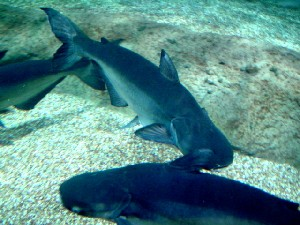
\includegraphics[width=7cm]
			        {wels.jpg}
			    \caption{Ein Wels.}
			\end{wrapfigure}
			Der Mekong-Riesenwels (Pangasianodon
			gigas) ist die größte Art der
			Familie der Haiwelse...
			\end{lstlisting}
			\column{0.5\textwidth}
			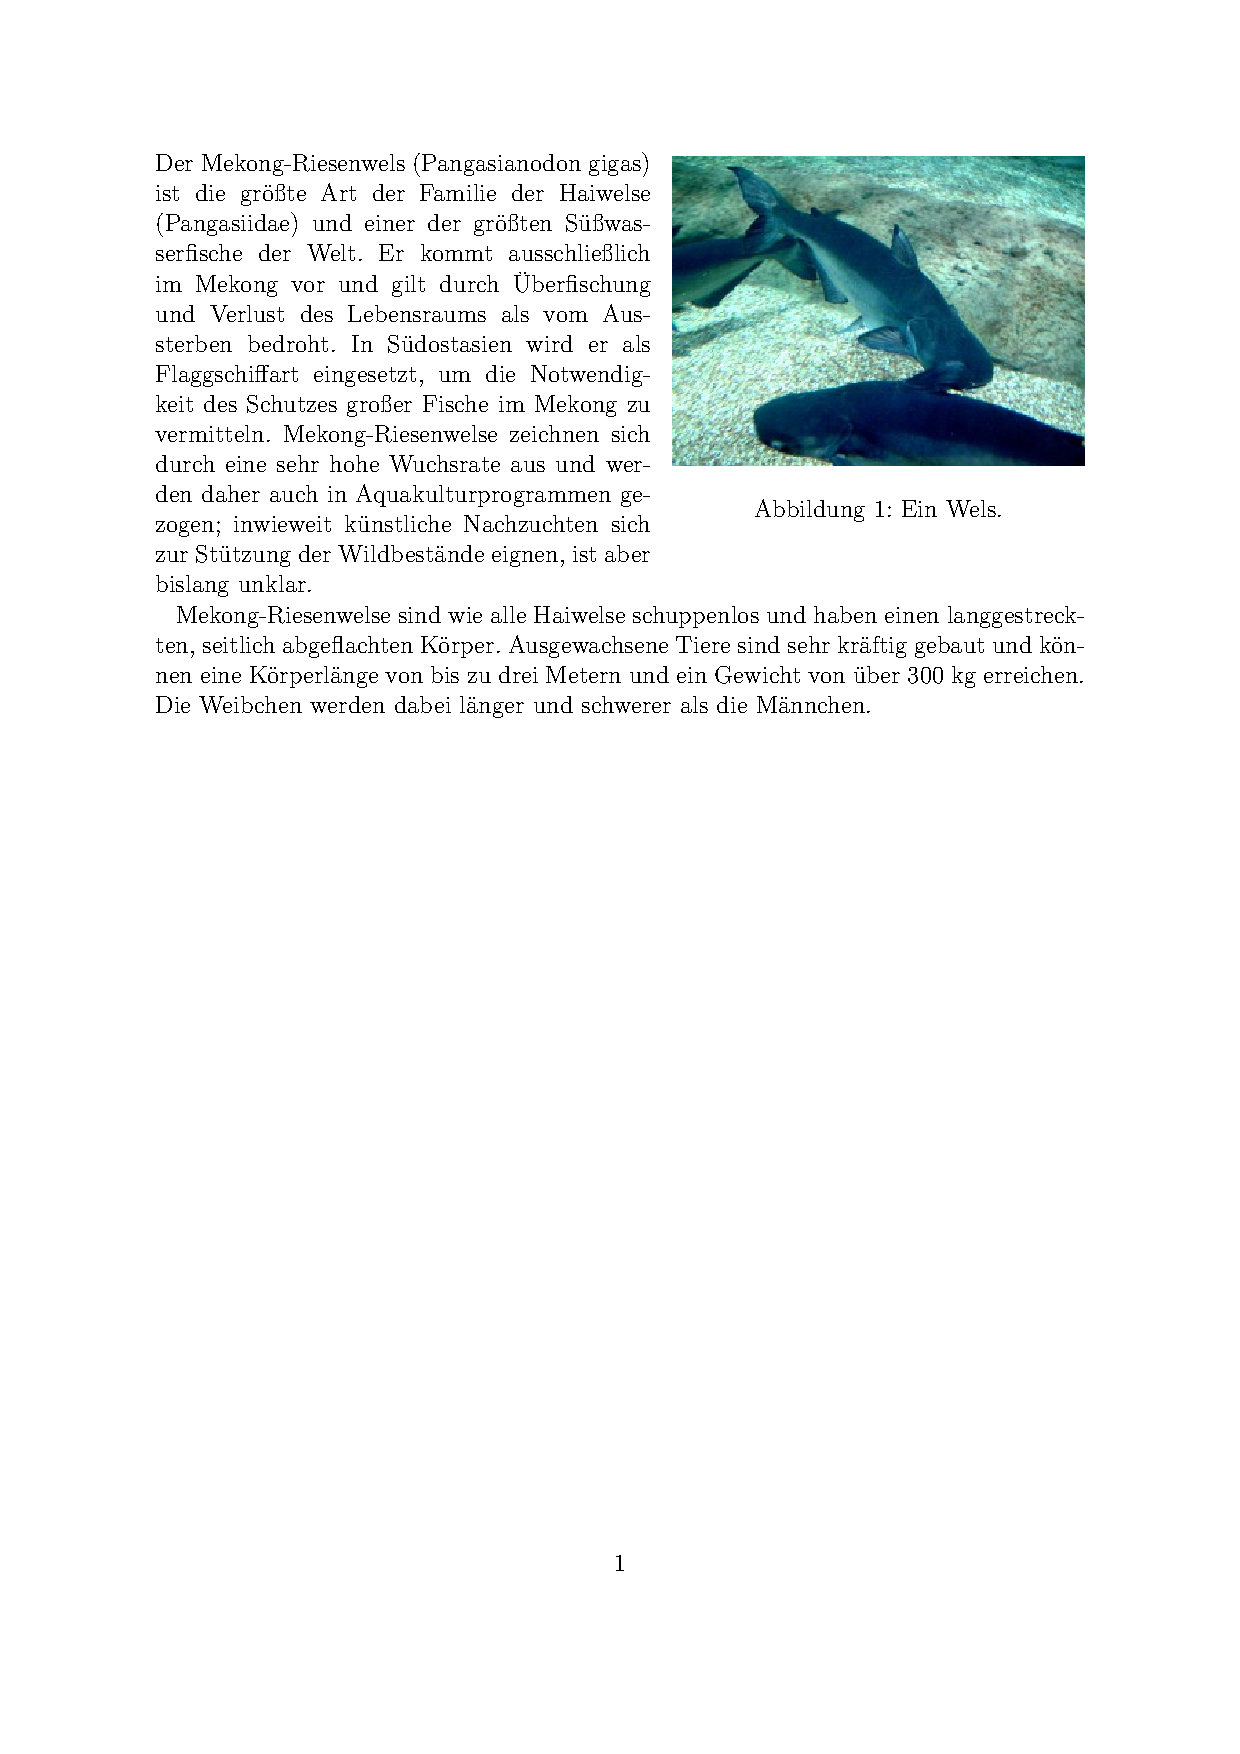
\includegraphics[width=\textwidth, trim=2cm 17cm 2cm 2cm, clip]{res/wrapfig_example.pdf}
		\end{columns}
		\item Bei Breite = \texttt{0cm}: Breite wird automatisch bestimmt
		\item Optional: \lstinline!\begin{wrapfigure}[<zeilen>]{<pos>}{<breite>} ... \end{wrapfigure}!
		
		Legt Zahl der Zeilen fest, die eingerückt werden sollen
	\end{itemize}
\end{frame}

\begin{frame}[<+->][fragile]
	\frametitle{Einheiten und Messwerte mit \texttt{siunitx}}
	\begin{itemize}
		\item Konfigurierbare und automatische Ausgabe von Werten mit Einheiten
		\item Verarbeitet auch Messunsicherheiten!
		\item \lstinline!\SI{zahl}{einheit}!, \lstinline!\num{zahl}!, \lstinline!\si{einheit}!
		\item \lstinline!\SI{5.42}{\m\per\s\squared}!
		\WarningFilter{latexfont}{Font shape}%
		\textrightarrow\ {\rmfamily\SI{5.42}{\m\per\s\squared}}
		\DeactivateWarningFilters
		\item Auch möglich (aber Anzeige nicht konfigurierbar):\\
		\lstinline!\SI{3,14}{m/s^2}! \textrightarrow\ {\rmfamily\SI{3,14}{m/s^2}}
		\item Eingabe von Punkt oder Komma als Dezimalseparator ist egal, es kommt das Richtige heraus
		\item Gruppierung von langen Zahlen: \lstinline!\num{9461846582}! \textrightarrow\ {\rmfamily\num{9461846582}}
		\item scientific notation: \lstinline!\SI{1,5e4}{\m}! \textrightarrow\ {\rmfamily\SI{1,5e4}{\m}}
		\item Unsicherheiten: \lstinline!\SI{2,71 +- 0,2}{\cm}! \textrightarrow\ {\rmfamily\SI{2,71 +- 0,2}{\cm}}
		\item Intervalle: \lstinline!\SIrange{400}{800}{\nm}! \textrightarrow\ {\rmfamily\SIrange{400}{800}{\nm}}
		\item Auflistungen:\\
		\lstinline!\SIlist{100; 200; 250}{\MHz}! \textrightarrow\ {\rmfamily\SIlist{100; 200; 250}{\MHz}}
	\end{itemize}
\end{frame}

\begin{frame}[<+->][fragile]
	\begin{itemize}
		\item Befehle für Einheiten: Häufige Einheiten sind vordefiniert (z.\,B.\ \lstinline!\cm!, \lstinline!\MHz!)
		\item Ansonsten: Basiseinheit mit Präfix: \lstinline!\MHz! = \lstinline!\mega\Hz!
		\item Quotienten: \lstinline!\per!, Potenzen: \lstinline!\squared!, \lstinline!\cubed!, \lstinline!\tothe{zahl}!
		\item Falls es nicht klappt: Einfach direkt eingeben
		\item Ausrichten von Zahlen in einer Tabelle: \lstinline!S!-Spalte
		\begin{columns}<.->
			\lstset{basicstyle=\footnotesize\ttfamily}
			\hspace{0.5cm}
			\column<.->{0.52\textwidth}
			\begin{lstlisting}
			\begin{tabular}{S S}
			\hline
			{Reihe 1 / \si{\kV}}
			    & {Reihe 2 / \si{\mA}} \\ \hline
			1,23	& 45,6 \\
			1,234	& 345,6 \\
			1,2345	& 2345,6 \\ \hline
			\end{tabular}
			\end{lstlisting}
			\column{0.45\textwidth}
			\rmfamily
			\begin{tabular}{S S}
			\hline
			{Reihe 1 / \si{\kV}}
			    & {Reihe 2 / \si{\mA}} \\ \hline
			1,23	& 45,6 \\
			1,234	& 345,6 \\
			1,2345	& 2345,6 \\ \hline
			\end{tabular}
		\end{columns}
		\item \emph{Falsch:} "{\rmfamily Es wurde eine Frequenz von $10,28 Hz$ gemessen}"
		
		\emph{Richtig:} "{\rmfamily Es wurde eine Frequenz von \SI[detect-family=true]{10,28}{Hz} gemessen}"
	\end{itemize}
\end{frame}

\begin{frame}[<+->][fragile]
	\frametitle{Unter-Abbildungen und -Tabellen mit \texttt{subcaption}}
	\begin{itemize}
		\item Wird verwendet, um mehrere Abbildungen mit eigenenen \lstinline!\caption{...}!s nebeneinander bzw.\ untereinander darzustellen
		\item Nummerierung: Abbildung 1 a), Abbildung 1 b), \dots
		\item \lstinline!\begin{subfigure}[<pos>]{<breite>} ... \end{subfigure}!\\
		und\\
		\lstinline!\begin{subtable}[<pos>]{<breite>} ... \end{subtable}!
		\item \lstinline!<pos>!: \lstinline!c!, \lstinline!b! oder \lstinline!t!
	\end{itemize}
\end{frame}


\begin{frame}[<+->][fragile]
	\begin{columns}<.->
		\lstset{basicstyle=\footnotesize\ttfamily, frame=L, numbers=left, xleftmargin=0.5cm}
		\column{0.55\textwidth}
		\begin{lstlisting}
		\begin{figure}
		    \begin{subfigure}{0.45\textwidth}
		        \centering\LARGE$\Phi$
		        \caption{Eine Abbildung.}
		    \end{subfigure}
		    % keine Leerzeile
		    % -> nebeneinander
		    \begin{subfigure}{0.45\textwidth}
		        \centering\LARGE$\Xi$
		        \caption{Eine weitere
		            Abbildung.}
		    \end{subfigure}
		    
		    \caption{Die gesamte Abbildung.}
		\end{figure}
		\end{lstlisting}
		\column{0.44\textwidth}
		\begin{figure}
			\subfloat[Eine Abbildung.]{%
			\begin{minipage}{0.45\textwidth}
		        \centering\LARGE$\Phi$
		    \end{minipage}}
		    % keine Leerzeile
		    % -> nebeneinander
			\subfloat[Eine weitere Abbildung.]{%
			\begin{minipage}{0.45\textwidth}
				\centering\LARGE$\Xi$
			\end{minipage}}

			\caption{Die gesamte Abbildung.}
		\end{figure}
	\end{columns}
	
	\bigskip
	\visible<+->{\emph{Wichtig:} \lstinline!subfigure! bzw.\ \lstinline!subtable! verhält sich wie ein in den Fließtext eingefügtes Bild \textrightarrow\ auf Leerzeilen (=~Absätze) achten}
\end{frame}

\section{\hologo{BibTeX}}

\begin{frame}[<+->][fragile]
	\frametitle{Bibliographie mit \hologo{BibTeX}}
	
	\lstset{frame=L, numbers=left,
		morekeywords={@book}, moreemph={title, author, isbn, series, url, year, publisher}}
	\begin{itemize}
		\item \lstinline!\usepackage{biblatex}!
		\item Informationen zu Literatur (Autor, Titel, Jahr etc.) werden in \texttt{.bib}-Dateien gespeichert
		\item Beispiel:
		\begin{lstlisting}
		@book{nolting2011grundkurs,
		    title = {Grundkurs Theoretische Physik 3: Elektrodynamik},
		    author = {Nolting, W.},
		    isbn = {9783642134494},
		    series = {Grundkurs Theoretische Physik},
		    url = {http://books.google.de/books?id=HOIfBAAAQBAJ},
		    year = {2011},
		    publisher = {Springer}
		}
		\end{lstlisting}
	\end{itemize}
\end{frame}

\begin{frame}[<+->][fragile]
	\lstset{frame=L, numbers=left,
		morekeywords={@book}, moreemph={title, author, isbn, series, url, year, publisher}}
	\begin{itemize}
		\item Beispiel:
		\begin{lstlisting}
		@book{nolting2011grundkurs,
		    title = {Grundkurs Theoretische Physik 3: Elektrodynamik},
		    author = {Nolting, W.},
		    isbn = {9783642134494},
		    series = {Grundkurs Theoretische Physik},
		    url = {http://books.google.de/books?id=HOIfBAAAQBAJ},
		    year = {2011},
		    publisher = {Springer}
		}
		\end{lstlisting}
		\item Mit (z.\,B.) \lstinline!\autocite{<name>}! oder \lstinline!\footcite{<name>}! wird zitiert
		\item "\lstinline!Nolting\footcite[Seite 42]{nolting2011grundkurs}!" \textrightarrow~"Nolting\footcite[Seite 42]{nolting2011grundkurs}"
	\end{itemize}
\end{frame}

\begin{frame}[<+->]
	\begin{itemize}
		\item Aufrufen eines \hologo{BibTeX}-kompatiblen Programms notwendig; Editoren wie TeXStudio erledigen dies automatisch
		\item Automatisches Literaturverzeichnis!
		\item Literaturangabe wird oftmals im \hologo{BibTeX}-Format zur Verfügung gestellt (z.\,B.\ Google Books – \url{https://books.google.com})
	\end{itemize}
	
	\visible<+->{
	\begin{center}
		\fbox{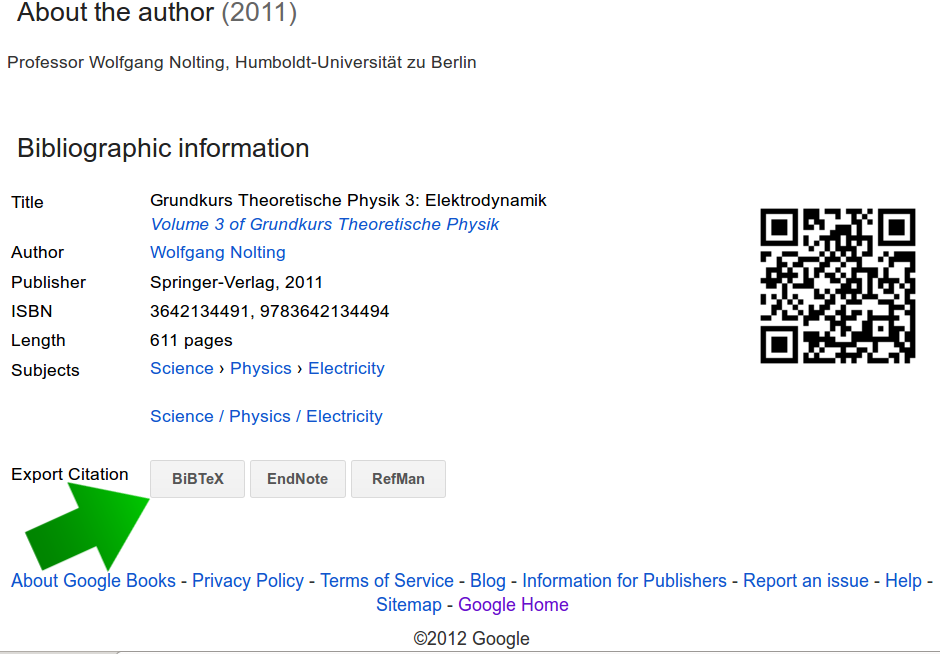
\includegraphics[width=0.65\textwidth]{res/nolting_google_books.png}}
	\end{center}
	}
\end{frame}

\begin{frame}[<+->]
	\frametitle{Literaturverzeichnis (Beispiel)}
	\nocite{sakurai2014modern}
	\printbibliography
	
	\hrule\bigskip
	
	Verwendete Werke erscheinen automatisch im Literaturverzeichnis.
\end{frame}

\section{Weitere Infos und Selbsthilfe}

\begin{frame}[<+->]
	\frametitle{Weitere Infos und Selbsthilfe}
	
	\begin{description}
		\item[\LaTeX-Wikibook] Hilfreiches \LaTeX-Tutorial (englisch)
		
		\url{https://en.wikibooks.org/wiki/LaTeX}
		\item[CTAN] "Comprehensive TeX Archive Network": Katalog aller bekannter \LaTeX-Pakete inkl.\ Dokumentation (meist PDF)
		
		\url{https://www.ctan.org}
		\item[FAQ-Listen] \url{http://projekte.dante.de/DanteFAQ} (deutsch)
		
		\url{http://www.tex.ac.uk} (englisch)
		\item[\TeX\ Stack Exchange] Q\,\&\,A-Seite zu \TeX\ und \LaTeX\ (englisch); bei spezifischen Problemen: Suchen oder selbst eine Frage stellen
		
		\url{https://tex.stackexchange.com}
		\item[\texttt{golatex.de}] \LaTeX-Forum (deutsch)
		
		\url{http://golatex.de}
		\item[Offizielle \LaTeX-Hilfe-Sammlung] Anleitungen auf der offiziellen \LaTeX-Seite
		
		\url{http://latex-project.org/guides}
	\end{description}
\end{frame}

\begin{frame}[<+->]
	\begin{description}
		\item[DANTE e.\,V.] \TeX-Anfänger-Seite von DANTE (Deutschsprachige Anwendervereinigung \TeX\ e.\,V.) 
		
		\url{http://www.dante.de/tex/TeXAnfaenger.html}
	\end{description}
	\visible<+->{\textbf{Andere Vorlagen/Hilfeseiten zum Praktikum:}}
	\begin{description}
		\item[Prof.\ Donath] Seite von Prof.\ Donath zum Grundpraktikum
		
		\url{https://www.uni-muenster.de/Physik.PI/Donath/Studieren/anleitung_experimentelle_uebungen.html}
		\item[Protokoll-Vorlage] \LaTeX-Vorlagen zu Protokollen und Abschlussarbeiten von Michael Entrup (AG Kohl) auf GitHub
		
		\url{https://github.com/m-entrup/LaTeX-Vorlagen}
		\item[Vorlage der Fachschaft Physik Karlsruhe] Vorlage für Protokolle in Karlsruhe (nicht getestet, aber evtl.\ gut als Vergleich)
		
		\url{https://fachschaft.physik.kit.edu/drupal/content/latex-vorlagen}
	\end{description}
\end{frame}

\begin{frame}[<+->]
	\frametitle{Materialien vom \LaTeX-Kurs}
	
	\centering
	\large
	
	\textbf{Unsere Vorlage für Protokolle und diese Folien}\\
	gibt es gleich oder unter
	
	\medskip
	\url{https://www.uni-muenster.de/imperia/md/content/physik_fsphys/latex-kurs/dateien_teilnehmer_2015.zip}
	
	\medskip
	
\includegraphics[width=0.4\textwidth]{res/qrcode_dateien.pdf}
\end{frame}

\section{gnuplot}
\subsection{Einführung}

\begin{frame}[<+->]
	\frametitle{gnuplot}
	\begin{itemize}
		\item Programm zum Zeichnen von Funktionen und zur Darstellung von Daten mit sehr (!) vielen Funktionen
		\item Kann insbesondere auch "Fit"-Funktion aus Messpunkten berechnen
		\item Textbasiert \textrightarrow\ Befehlseingabe über die Kommandozeile
		\item Ausgabe der Diagramme in vielen Formaten, z.\,B.\ PDF
		
		\textrightarrow\ Einbinden in \LaTeX-Dokumente
		\item Leider etwas gewöhnungsbedürftige Mathe-Syntax\dots\footnote<.->{Fortran-ähnlich; werdet ihr im 4.\ Semester noch genauer kennenlernen\dots}
		\item Zum Nachlesen: \textbf{Gnuplot-Dokumentation} (PDF) auf\\
		\url{http://gnuplot.info/documentation.html} (sehr ausführlich!)
		\item Sehr viele \textbf{Beispiele} (Bilder und Code!) gibt es unter\\
		\url{http://www.gnuplot.info/screenshots}
	\end{itemize}
\end{frame}

\subsection{Beispiel}

\begin{frame}[<+->]
	Wichtigste Befehle:
	\begin{description}
		\item[\texttt{set <option> [wert]}] Setzen von Einstellungen (meist Darstellung)
		\item[\texttt{plot <funktion\_oder\_werte> [optionen]}] Zeichnet Funktionen oder Messwerte
		\item[\texttt{fit <funktion> <werte> [optionen]}] Versucht, Parameter zu berechnen, sodass die Funktion möglichst gut zu den Messwerten passt
	\end{description}

	\begin{columns}<.->
		\column{0.2\textwidth}
		Beispiel:
		\column<.->{0.7\textwidth}
		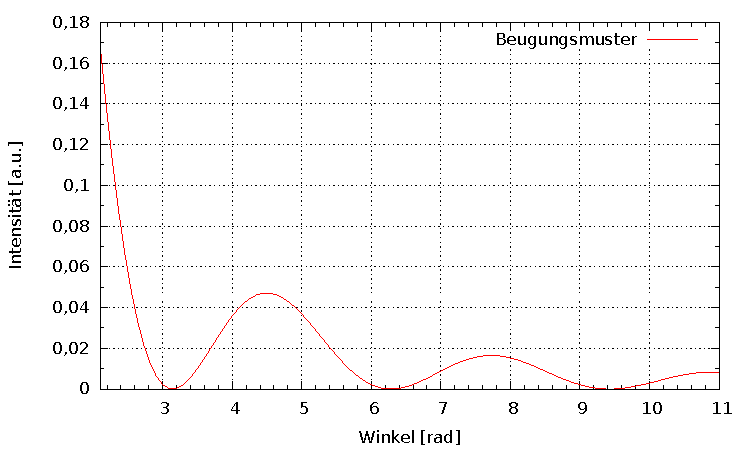
\includegraphics[width=\textwidth]{res/beispiel.pdf}
	\end{columns}
\end{frame}

\begin{frame}[<+->]
	Wie wurde der Graph erzeugt?

	\lstset{frame=L, numbers=left, xleftmargin=0.6cm}
	\lstset{language=Gnuplot, morekeywords={decimalsign}}
	\begin{columns}
		\column{0.7\textwidth}
		\lstinputlisting{res/gnuplot.gp}
		\column{0.29\textwidth}
		\hspace*{-2.2cm}
		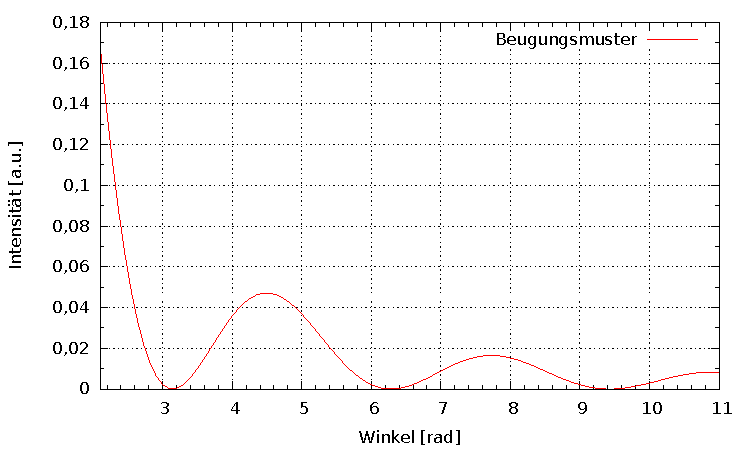
\includegraphics[width=1.6\textwidth]{res/beispiel.pdf}
		\vspace*{-2cm}
	\end{columns}
\end{frame}

\subsection{Syntax}

\begin{frame}[<+->][fragile]
	\frametitle{Syntax}
	\lstset{language=Gnuplot, moreemph={pi}, literate={}}
	\begin{itemize}
		\item Kommentare mit \lstinline|#|
		\item Pro Zeile ein Befehl (oder mehrere pro Zeile mit Semikolon getrennt)
		\item Definition eines Wertes/einer Funktion:
		\begin{lstlisting}
		# Einige Definitionen
		zahl = 5.4
		funktion(var1, var2, a) = sqrt(var1 - var2) + a**2
		\end{lstlisting}
		\item Es gibt viele eingebaute Funktionen (\lstinline|pi|, \lstinline|sqrt(x)|, \lstinline|sin(x)|, \lstinline|atan(x)|, \lstinline|erf(x)|\dots)
		\item Zeichnen einer Funktion:
		\begin{lstlisting}
		# Variable ist immer x!
		# "with ..." gibt Art der Darstellung ("plotting style") an
		plot f(x) with lines title 'Legende'
		\end{lstlisting}
	\end{itemize}
\end{frame}

\begin{frame}[<+->][fragile]
	\lstset{language=Gnuplot, literate={}}
	\begin{itemize}
		\item Zeichnen von Datenpunkten:
		\begin{lstlisting}
		# "using" wählt Spalten aus (1. Spalte: x, 2. Spalte: y)
		plot 'datei1.csv' using 1:3 with linespoints title 'Daten'
		# Manche Darstellungsarten brauchen mehr Spalten
		plot 'datei2.csv' using 1:3:5:6 with xyerrorbars
		# Klammern bei "using" erlauben Berechnungen
		# "$1" steht dann für den Wert der 1. Spalte usw.
		plot 'datei3.csv' using (2 * $1):(sqrt($4) + 42)
		\end{lstlisting}
		
		\visible<+->{\textbf{Achtung bei Division!} Gnuplot verwendet standardmäßig Integer-Division, d.\,h.\ \lstinline|1/2|~=~\lstinline|0|!
		
		\textrightarrow~Zur Sicherheit immer Kommazahlen verwenden: \lstinline|1./2.|~=~\lstinline|0.5|}
		\item Mehrere Plots in einem Graphen durch Kommas:
		\begin{lstlisting}
		plot 'datei.csv' using 1:2 title 'Daten', g(x) + 3 title 'Fit', exp(3 * sin(x)) + x**3 title 'Theorie'
		\end{lstlisting}
	\end{itemize}
\end{frame}

\begin{frame}[<+->][fragile]
	\lstset{language=Gnuplot, literate={}}

	Beispiel für Fit:
	\begin{lstlisting}
	fit m*x + b 'datei.csv' using 1:2 via m, b
	\end{lstlisting}
	
	\textbf{Vorsicht} bei nichtlinearen Fits: Es kann sein, dass gnuplot keinen guten Fit findet (Fit-Fehler)\\
	\textrightarrow~Sinnvolle Startwerte für Parameter angeben!
	\begin{lstlisting}
	m = 10
	b = 4.1e4 # = 41000
	fit m*x + b 'datei.csv' using 1:2 via m, b
	\end{lstlisting}

	\centering
	\begin{columns}<.->
		\column{0.35\textwidth}
		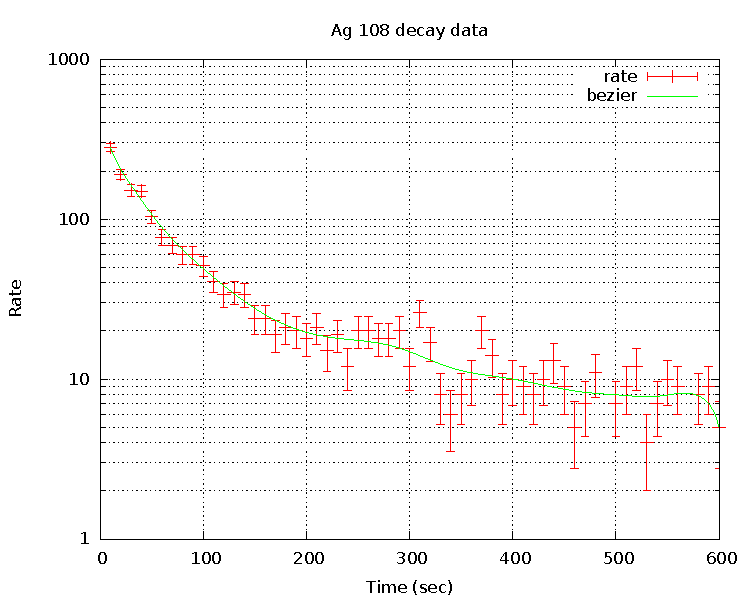
\includegraphics[width=\textwidth]{res/gnuplot_silver.pdf}
		\hspace*{-0.02\textwidth}
		\column{0.35\textwidth}
		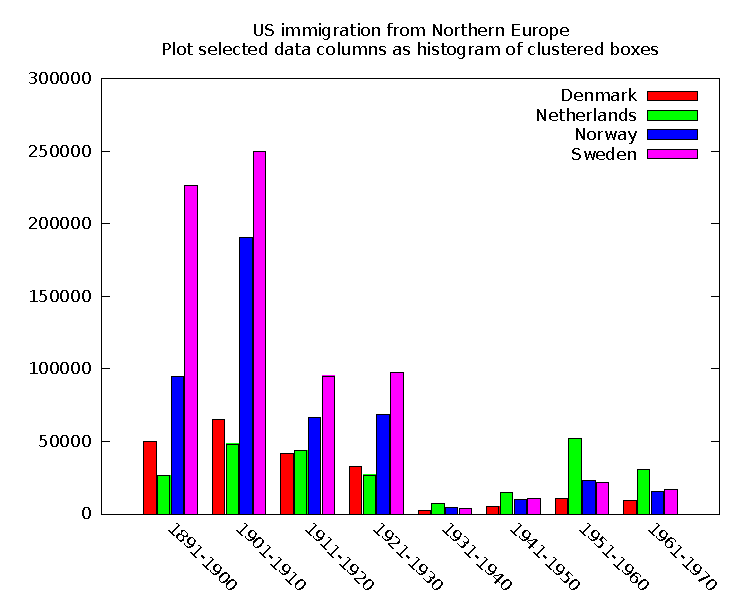
\includegraphics[width=\textwidth]{res/gnuplot_histogram.pdf}
		\hspace*{-0.02\textwidth}
		\column{0.35\textwidth}
		\hspace*{-0.02\textwidth}
		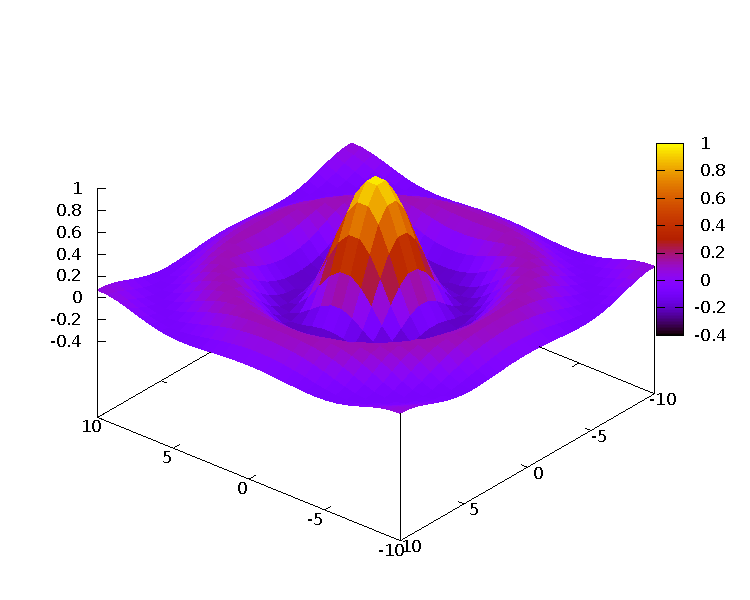
\includegraphics[width=\textwidth]{res/gnuplot_pm3d.pdf}
	\end{columns}
\end{frame}

\section*{}
\subsection*{}

\begin{frame}
	\begin{block}{}
		\centering
		Vielen Dank für eure Aufmerksamkeit!
	\end{block}

	\begin{block}{}
		\centering
		Habt ihr noch Fragen?
	\end{block}
	
	\begin{block}{}
		\centering\LARGE
		Nach dem Mittagessen: Treffen im ZIV!
	\end{block}

	\begin{center}
		
\includegraphics[width=7cm]{res/logo.pdf}
		
		\medskip
		\url{https://www.uni-muenster.de/Physik.FSPHYS}
	\end{center}
\end{frame}

\end{document}
